%!TeX program = xelatex
\documentclass{SYSUReport}

\usepackage{float}
\usepackage{longtable}
\usepackage{array}
\usepackage{tabularx}
\usepackage{caption}
\usepackage{xurl}

\headl{多智能体系统设计与实现}
\headr{人工智能实验}
\lessonTitle{人工智能实验}
\reportTitle{南郭先生们：多智能体音乐创作系统}
\inst{计算机学院}
\major{保密管理}
\stuname{吕梓文}
\stuid{24353028}
\date{2026年7月}

\setlength{\parindent}{2em}
\setlength{\parskip}{0.25em}
\setlength{\headheight}{15pt}
\renewcommand{\arraystretch}{1.28}
\newcolumntype{Y}{>{\raggedright\arraybackslash}X}
\newcolumntype{L}[1]{>{\raggedright\arraybackslash}p{#1}}

\begin{document}

\cover
\updateheader{南郭先生们：多智能体音乐创作系统}
\thispagestyle{empty}
\clearpage

\begin{abstract}
本实验设计并实现了一个基于 LangGraph 的本地多智能体音乐创作系统“南郭先生们”。系统并不让单一大模型一次性生成全部内容，而是把音乐创作拆分为需求理解、工作流规划、作词、旋律、和声、节奏、即兴、演奏、编曲、音色设计、混音审查和生成提示词编译等职责，再依据作品类型组合成不同的乐团工作流。对外的“南郭先生”负责多轮对话、作品协调与记忆读取；Conductor Agent 依据当前请求和有效偏好选择受约束的预设路径；各专业 Agent 通过 Pydantic 结构化状态逐步交接领域结果；最后由供应商适配层调用 Suno 兼容服务并完成本地下载、音频分析和波形渲染。

系统实现了三种互补的推理组织方式：以 Conductor 为核心的受约束计划--执行、参考音频分析中的工具调用式 ReAct，以及生成前由 Mix Review Agent 完成的反思审查。记忆模块同时提供会话内短期记忆和跨会话长期记忆，并通过“显式创作参数、当前请求、长期偏好、系统默认”的优先级消解冲突。工具层则覆盖音频探测与变换、波形可视化、轻量 Demo 合成、MusicXML/MIDI 导出和外部音乐生成等多类能力。实验结果表明，系统能够在流行人声、古典器乐、电子器乐和影视配乐等场景下选择差异化路径，完成人机对话、后台生成、进度反馈、作品归档与偏好管理。报告最后结合实际界面与测试结果分析了其效果，并讨论参考音频理解深度、生成可控性、并发能力和版权风格约束等后续改进方向。

\textbf{关键词：}多智能体系统；LangGraph；音乐生成；结构化状态；长期记忆；工具调用
\end{abstract}

\clearpage
\tableofcontents
\clearpage
\pagenumbering{arabic}
\setcounter{page}{1}

\section{实验题目与目标}

\subsection{实验题目}

使用开源智能体编排框架设计并实现一个多智能体系统。实验选取“本地音乐创作工作台”作为任务场景，系统名称为“南郭先生们”（theNanGuos）：多个具有明确音乐职责的智能体组成南郭乐团，由对外代表与指挥智能体理解需求、安排分工，最终形成可播放、可下载、可恢复的音乐作品及其中间产物。

\subsection{实验目标}

本实验希望解决的核心问题不是“让模型写一段音乐提示词”，而是如何把一个开放、含糊且跨多个专业环节的音乐需求，转化为可检查、可组合、可执行的协作过程。具体目标如下：

\begin{enumerate}
    \item 设计不少于四个、职责边界清楚的智能体，使其提示词、输入字段和输出字段与任务相匹配；
    \item 以图工作流组织协作，根据流行人声、器乐、电子、影视配乐等任务动态选择节点，允许纯器乐路径跳过作词；
    \item 实现至少一种智能体推理或规划机制，并使规划结果受到系统白名单约束；
    \item 同时提供会话内短期记忆和跨会话长期记忆，保证当前明确需求优先于历史偏好；
    \item 接入至少两类工具能力，把语言模型不适合稳定完成的音频探测、文件变换、乐谱导出和服务调用交给确定性程序；
    \item 完成可本地运行的前后端系统，形成从创作输入到作品管理的闭环，并对实现效果进行实验分析。
\end{enumerate}

\section{需求分析与总体设计}

\subsection{任务特点}

音乐创作天然具有多阶段、强依赖和多解性。歌词必须服从主题与语言；旋律需要兼顾歌词重音、和声与节奏；编曲依赖此前形成的旋律、和声和动态计划；供应商提示词又不能混入内部 JSON、文件路径或过多解释。因此若让一个模型一次完成所有工作，通常会出现职责混杂、前后矛盾、器乐作品误生成人声、结果难以校验等问题。

系统据此采用“领域决策由智能体完成，机械操作由工具完成，外部服务由 provider 隔离”的原则。智能体只负责需要语义判断和音乐规划的内容；ffmpeg、ffprobe、music21 等承担确定性处理；KIE/Suno 请求集中在供应商适配层；FastAPI 与本地文件存储负责运行生命周期。该划分使每个环节都有清楚的输入、输出与失败位置。

\subsection{四层架构}

系统从上到下分为四层：

\begin{enumerate}
    \item \textbf{交互层}：React、TypeScript 与 React Flow 构成对话页、创作台、工作流画布、作品集和记忆库；
    \item \textbf{应用层}：FastAPI 处理会话、项目、上传、运行状态与作品接口，本地后台线程负责长时间生成任务；
    \item \textbf{智能体编排层}：LangGraph 管理条件分支，Pydantic/TypedDict 管理共享状态，各 Agent 只更新自己负责的字段；
    \item \textbf{能力层}：本地文件系统保存数据，音频与乐谱工具产生中间产物，独立 provider 对接 Suno 兼容服务。
\end{enumerate}

其核心数据流可概括为：

\begin{center}
用户请求/参考音频 $\rightarrow$ 会话与偏好解析 $\rightarrow$ Conductor 规划
$\rightarrow$ 专业 Agent 协作 $\rightarrow$ Prompt Compiler
$\rightarrow$ Demo/音乐生成 $\rightarrow$ 音频分析与作品归档。
\end{center}

图~\ref{fig:studio} 展示了系统的主要工作区。左侧输入作品名称、预设乐团、流派、语言、乐器、文字构想和参考音频；中央使用图展示智能体编排；右侧报告运行阶段；下方同时提供中间 Demo、最终音频、波形和提示词信息。它把内部图执行转换为用户能够理解和操作的创作流程。

\begin{figure}[H]
    \centering
    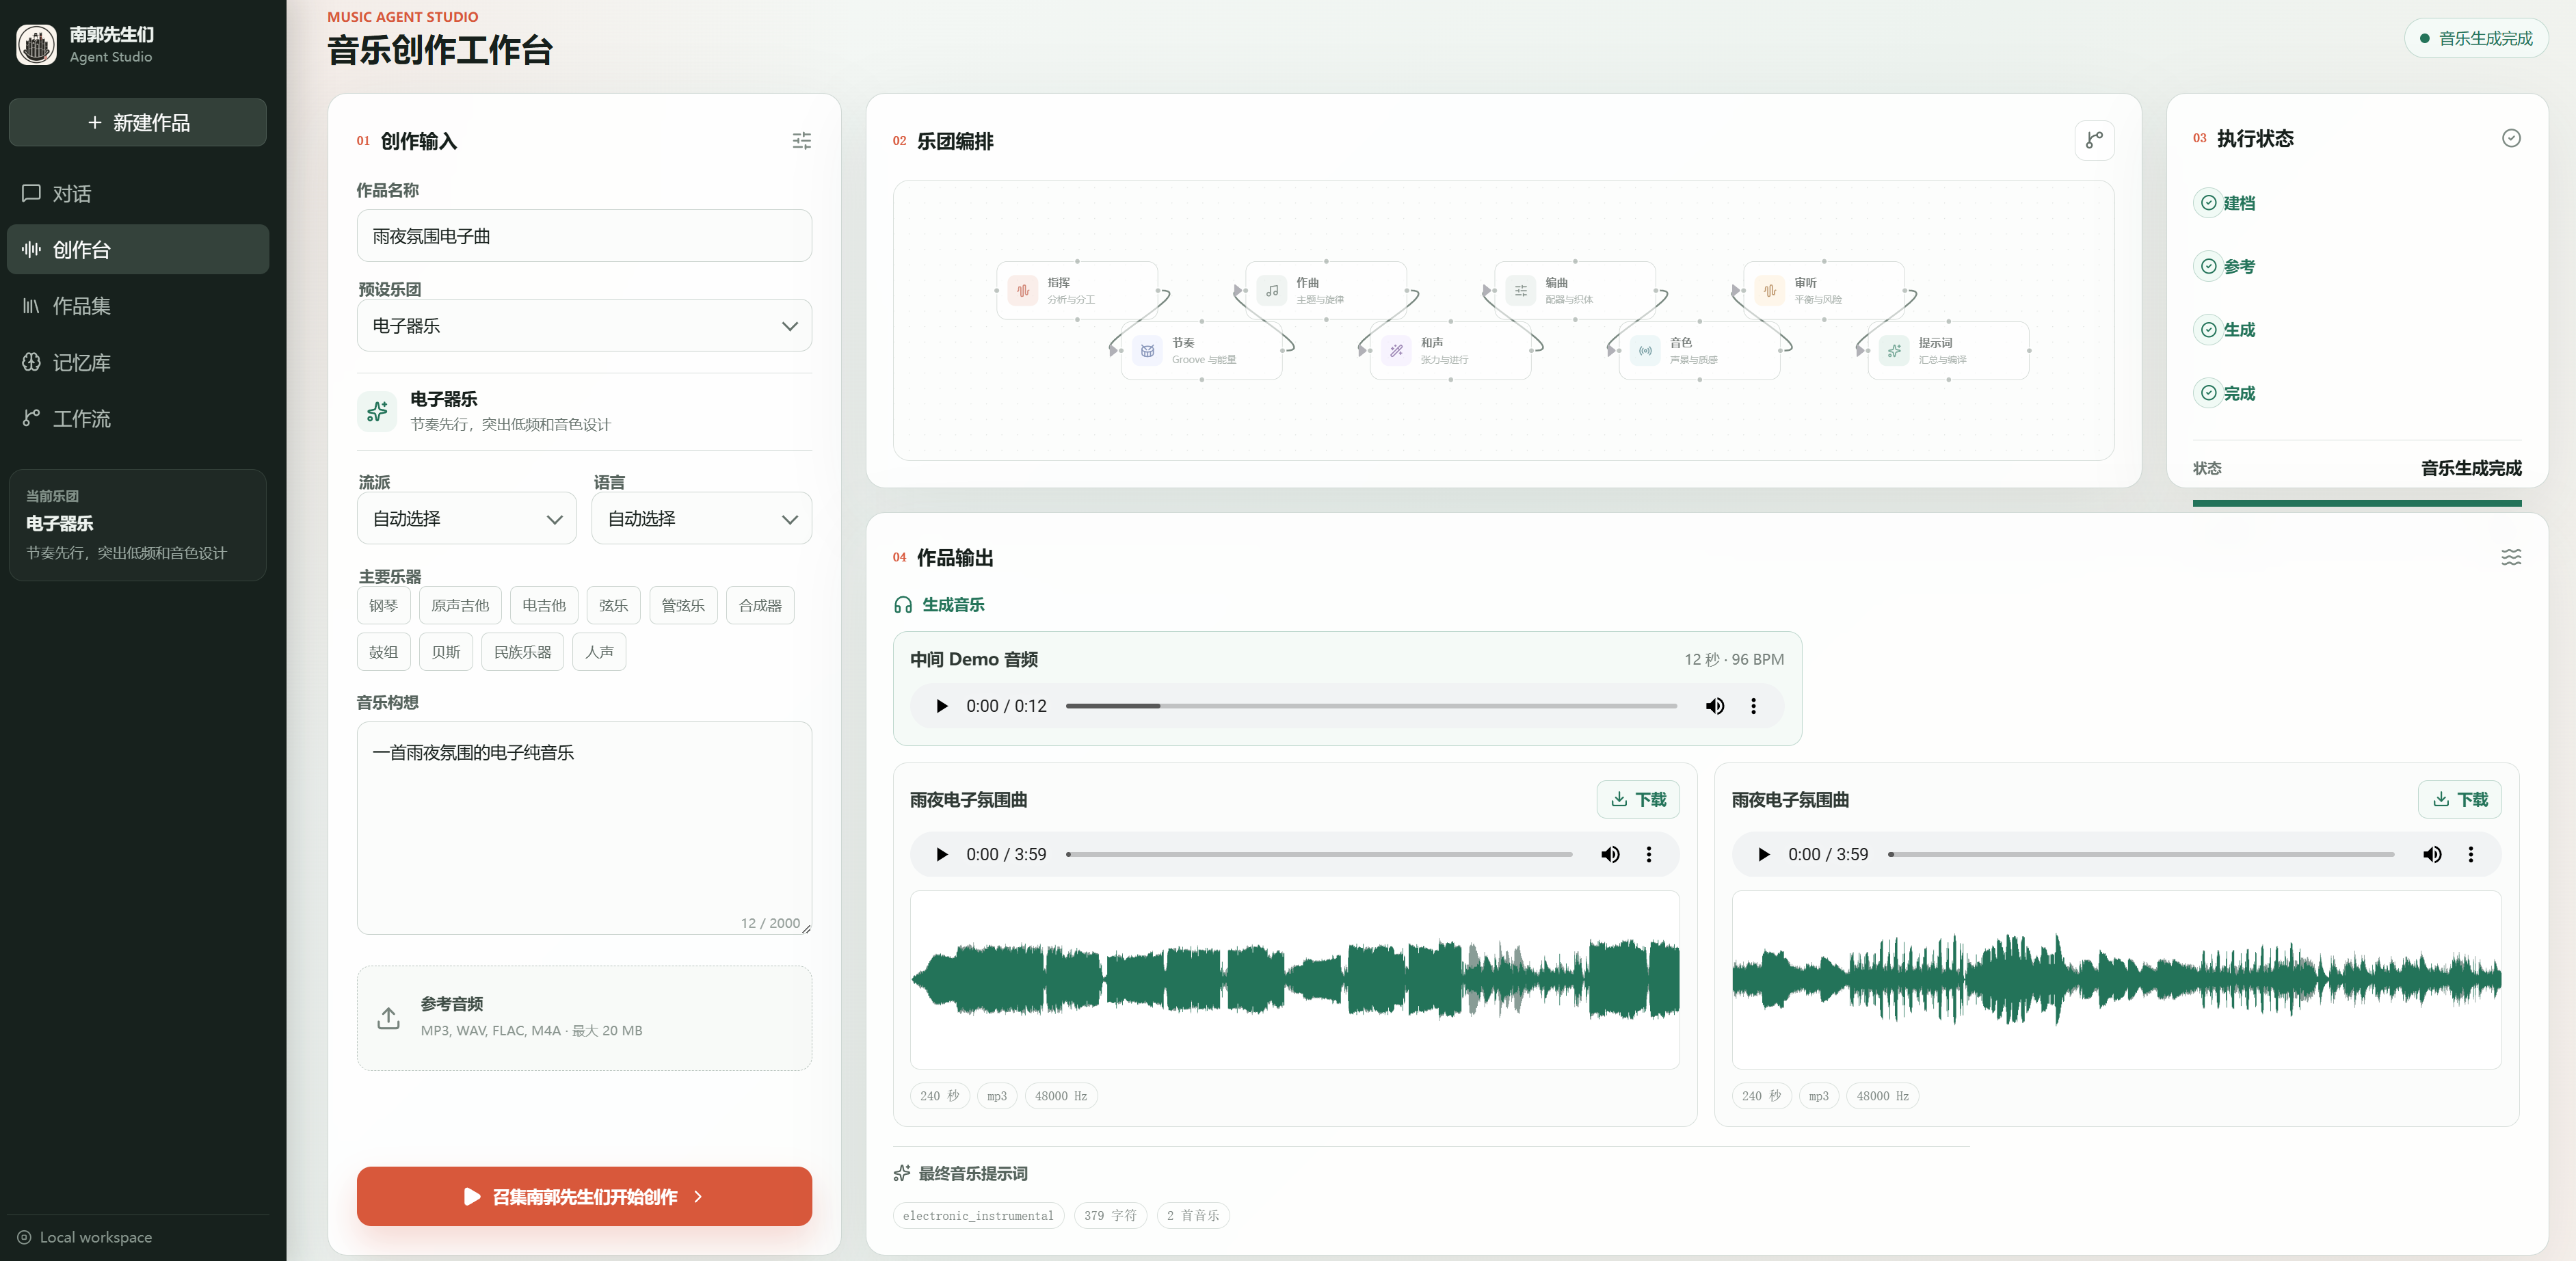
\includegraphics[width=\textwidth]{images/创作台.png}
    \caption{音乐创作工作台总览}
    \label{fig:studio}
\end{figure}

\subsection{技术选型}

\begin{table}[H]
    \centering
    \caption{主要技术及其职责}
    \label{tab:stack}
    \begin{tabularx}{\textwidth}{L{3.0cm}L{3.3cm}Y}
        \toprule
        技术 & 所在层次 & 采用原因与职责 \\
        \midrule
        Python 3.12、uv & 基础环境 & 统一依赖解析、虚拟环境和运行命令，降低本地复现实验的成本。 \\
        LangGraph & 智能体编排 & 以 StateGraph 表达节点、条件边和终止条件，适合可组合的多分支流程。 \\
        Pydantic & 数据边界 & 为创意简报、歌词、旋律、乐谱、记忆和运行结果提供校验，避免依赖自由文本解析关键字段。 \\
        FastAPI & 应用接口 & 提供类型明确的本地 REST API、上传和静态作品访问。 \\
        React/TS & 前端 & 构建对话、创作、记忆和作品管理界面；React Flow 显示执行路径。 \\
        ffmpeg/ffprobe & 音频工具 & 读取音频元数据，生成预览、波形和轻量 Demo。 \\
        music21 & 乐谱工具 & 根据受约束的 ScoreSpec 导出 MusicXML 与 MIDI。 \\
        KIE/Suno provider & 外部生成 & 把供应商鉴权、参数限制、轮询和下载与 Agent 职责隔离。 \\
        \bottomrule
    \end{tabularx}
\end{table}

\section{多智能体系统设计}

\subsection{角色划分与职责边界}

系统实际包含对话协调、参考分析、工作流规划和多个音乐专业角色，数量明显多于最低协作规模。每个角色并非仅有不同名称，而是具有独立系统提示词、限定输入字段和 Pydantic 输出模型。表~\ref{tab:agents} 给出各角色在完整链路中的定位。

\begin{longtable}{L{2.7cm}L{4.0cm}L{7.0cm}}
    \caption{智能体角色、输入和输出}\label{tab:agents}\\
    \toprule
    角色 & 主要读取内容 & 主要职责与结构化输出 \\
    \midrule
    \endfirsthead
    \toprule
    角色 & 主要读取内容 & 主要职责与结构化输出 \\
    \midrule
    \endhead
    南郭先生 & 当前消息、近期消息、会话摘要、记忆上下文、活动项目 & 进行自然对话，决定聊天、建项、生成、修改、查看作品或追问；提取明确偏好。 \\
    Audio Reference & 上传资产索引 & 通过白名单工具探测音频、生成短预览或波形，输出 AudioReference 列表。 \\
    Conductor & 用户请求、预设、记忆上下文、有效偏好 & 选择八种工作流之一，形成 CreativeBrief 和各角色指令。 \\
    Lyrics & 创意简报、用户请求、指挥指令 & 生成分段歌词、主题、Hook、语言和演唱提示；只出现在人声路径。 \\
    Melody & 简报、歌词、已有和声/节奏 & 规划速度、主题旋律、Hook 和情绪弧；必要时生成受约束 ScoreSpec。 \\
    Harmony & 简报、歌词、旋律 & 规划调性中心、和弦进行、和声节奏和张力策略。 \\
    Rhythm & 简报、歌词、旋律与和声 & 规划 Groove、打击乐、节奏动机和能量曲线。 \\
    Improvisation & 爵士路径中的和声、节奏、旋律 & 规划独奏者、solo 曲式、即兴语汇、合奏互动与边界。 \\
    Performance & 旋律、节奏、即兴计划 & 规划演奏法、力度、乐手关系和人性化细节。 \\
    Arrange & 前述音乐计划与音频参考 & 确定配器、段落发展、织体和制作方向。 \\
    Sound Design & 简报与编曲计划 & 规划音色调色板、标志性声音、空间运动和质感。 \\
    Mix Review & 全部主要音乐计划 & 在生成前审查平衡、低频、结构、风格漂移等风险，形成审听建议。 \\
    Prompt Compiler & 全部结构化创作结果、有效偏好 & 把领域计划压缩为少于 500 字符的供应商可用提示词。 \\
    \bottomrule
\end{longtable}

这种角色边界体现了“最小必要读取”原则。例如 Lyrics 不读取供应商配置，Prompt Compiler 不负责网络请求，KIE provider 也不参与音乐创意判断。角色之间交换的是 \texttt{LyricsDraft}、\texttt{MelodyPlan}、\texttt{HarmonyPlan} 等明确对象，而不是从上一角色的一段自然语言回复中猜测字段。

\subsection{结构化状态交接}

LangGraph 的共享 State 使用 TypedDict 声明可选字段，每种领域结果再由 Pydantic 模型约束。例如 CreativeBrief 把标题、语言、流派、情绪、主题、时长、速度、人声与结构统一成一个可校验对象；NoteEvent 对音高、时值和力度设定范围；最终提示词也有长度上限。每个通用 Agent wrapper 只根据 \texttt{input\_fields} 构造输入，并只返回输出模型定义的字段。

\noindent\textbf{代码 1：通用 Agent 的结构化输入输出机制（节选）}
\begin{minted}{python}
payload = {
    field: _json_value(state[field])
    for field in self.input_fields
    if field in state
}
runner = self.llm.with_structured_output(
    self.output_schema,
    method=method,
)
response = runner.invoke(messages)
response = self.output_schema.model_validate(response)
return {
    field: getattr(response, field)
    for field in type(response).model_fields
}
\end{minted}

当模型服务不支持原生 function calling/json schema 时，系统还可以切换到 prompt JSON 或 JSON mode，再用 Pydantic 做最终验证。若结构化输出仍失败，少数适合保底的音乐角色会返回最小可用方案；无法安全保底的角色则抛出包含失败阶段的错误，而不是把无效文本静默传给后续节点。

\subsection{可组合工作流}

系统注册了八种预设。它们复用同一组角色，但入口顺序和可选节点随音乐类型变化，如表~\ref{tab:workflows} 所示。

\begin{table}[H]
    \centering
    \small
    \caption{预设工作流的关键路径差异}
    \label{tab:workflows}
    \begin{tabularx}{\textwidth}{L{3.1cm}Y}
        \toprule
        工作流 & Audio Reference 和 Conductor 之后的主要节点 \\
        \midrule
        \path{pop_vocal} & Lyrics $\rightarrow$ Melody $\rightarrow$ Harmony $\rightarrow$ Rhythm $\rightarrow$ Arrange \\
        \path{classical_instrumental} & Melody $\rightarrow$ Harmony $\rightarrow$ Arrange $\rightarrow$ 可选 Score Export \\
        \path{electronic_instrumental} & Rhythm $\rightarrow$ Melody $\rightarrow$ Harmony $\rightarrow$ Arrange \\
        \path{soundtrack_score} & Melody $\rightarrow$ Harmony $\rightarrow$ Arrange \\
        \path{jazz_ensemble} & Harmony $\rightarrow$ Rhythm $\rightarrow$ Melody $\rightarrow$ Improvisation $\rightarrow$ Performance $\rightarrow$ Arrange \\
        \path{rock_vocal} & Lyrics $\rightarrow$ Melody $\rightarrow$ Harmony $\rightarrow$ Rhythm $\rightarrow$ Performance $\rightarrow$ Arrange \\
        \path{folk_acoustic} & Lyrics $\rightarrow$ Melody $\rightarrow$ Harmony $\rightarrow$ Performance $\rightarrow$ Arrange \\
        \path{hiphop_vocal} & Rhythm $\rightarrow$ Lyrics $\rightarrow$ Melody $\rightarrow$ Harmony $\rightarrow$ Performance $\rightarrow$ Arrange \\
        \midrule
        公共收尾 & Sound Design $\rightarrow$ Mix Review $\rightarrow$ Prompt Compiler \\
        \bottomrule
    \end{tabularx}
\end{table}

图~\ref{fig:pop-flow}--\ref{fig:soundtrack-flow} 对比了三种典型画布。流行人声先完成作词，再依次规划旋律、和声与节奏；嘻哈人声则把 Rhythm 放在 Lyrics 之前，先建立 beat 与 flow 的节奏骨架，并在编曲前增加 Performance 规划以控制说唱咬字、动态和人性化细节；影视配乐跳过作词及常规人声路径，围绕主题旋律、和声张力、配器和空间音色展开。画布显示面向用户的核心创作节点，后端实际执行还包括前置的参考音频分析。

\begin{figure}[H]
    \centering
    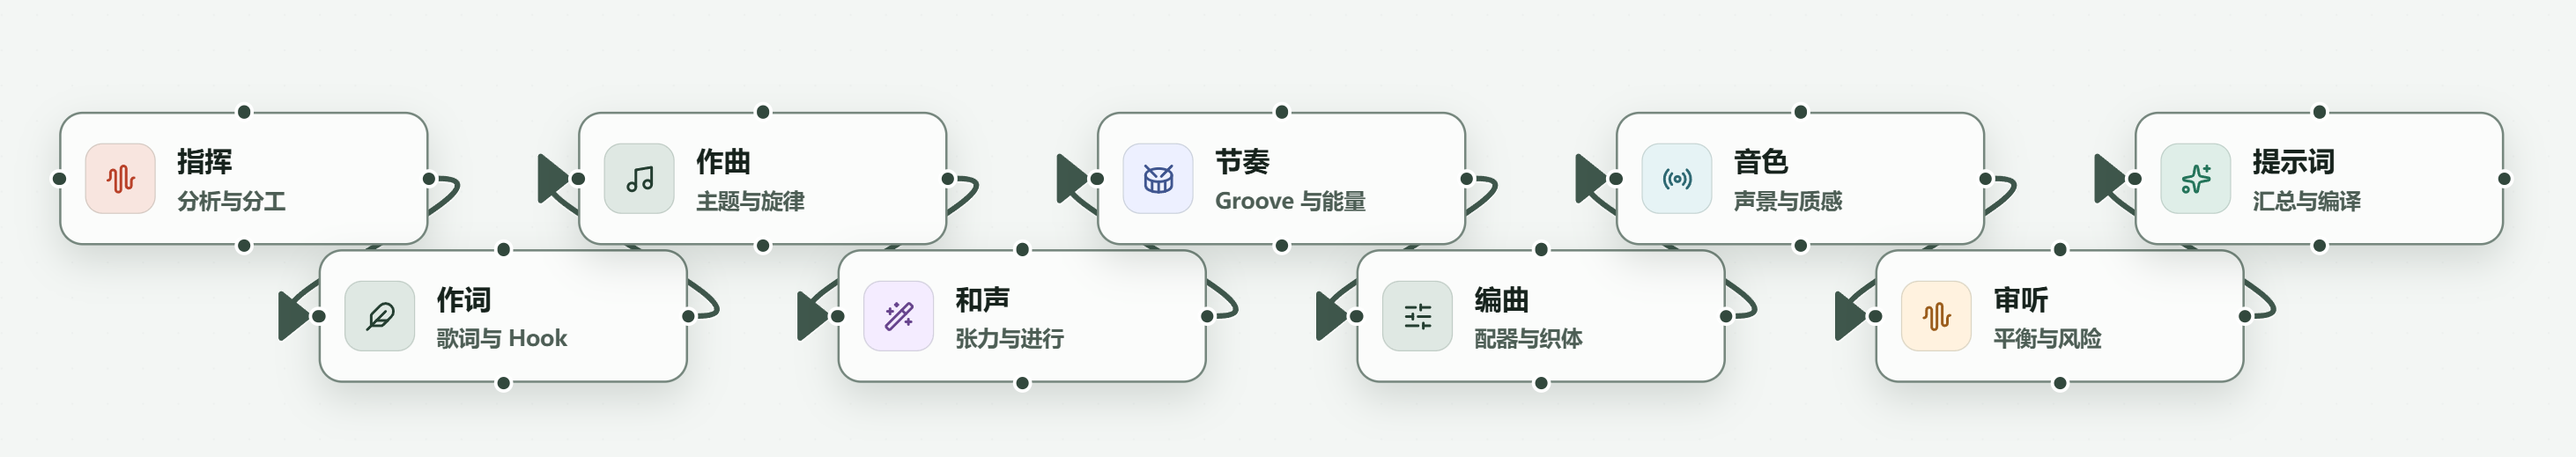
\includegraphics[width=\textwidth]{images/流行人声编排.png}
    \caption{流行人声工作流：作词节点参与协作}
    \label{fig:pop-flow}
\end{figure}

\begin{figure}[H]
    \centering
    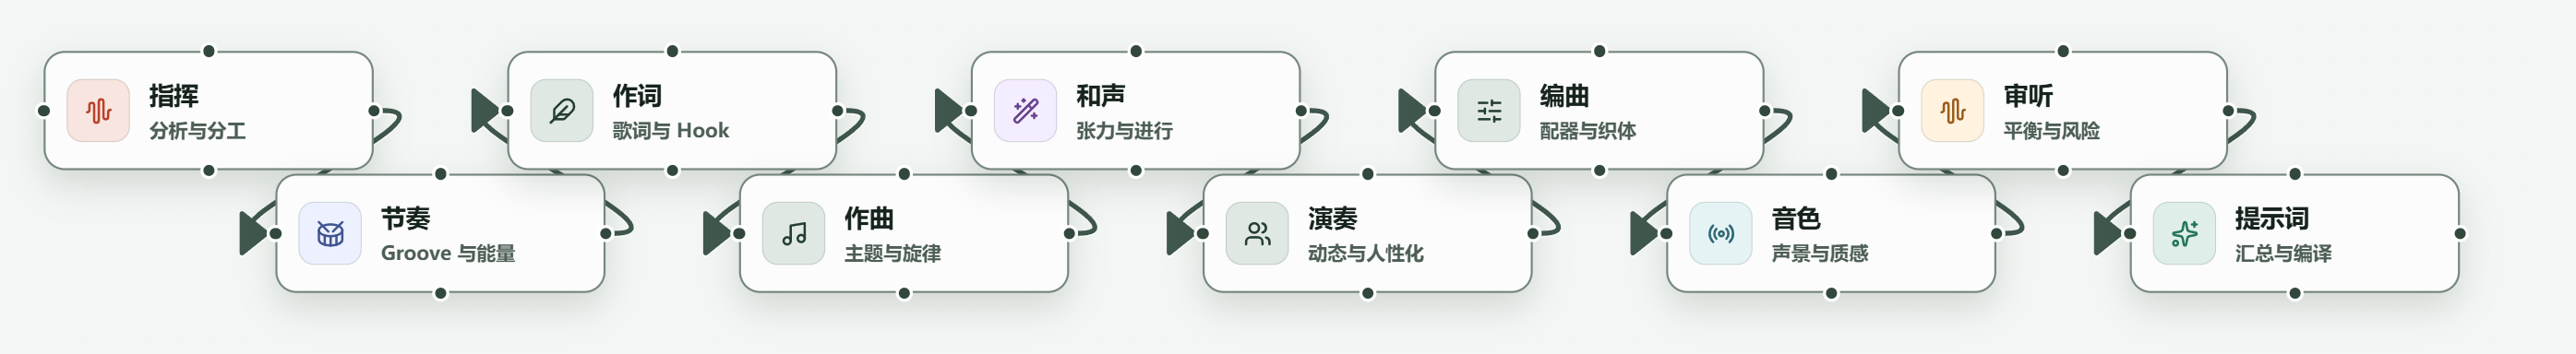
\includegraphics[width=\textwidth]{images/嘻哈人声编排.png}
    \caption{嘻哈人声工作流：节奏先行并加入演奏规划}
    \label{fig:hiphop-flow}
\end{figure}

\begin{figure}[H]
    \centering
    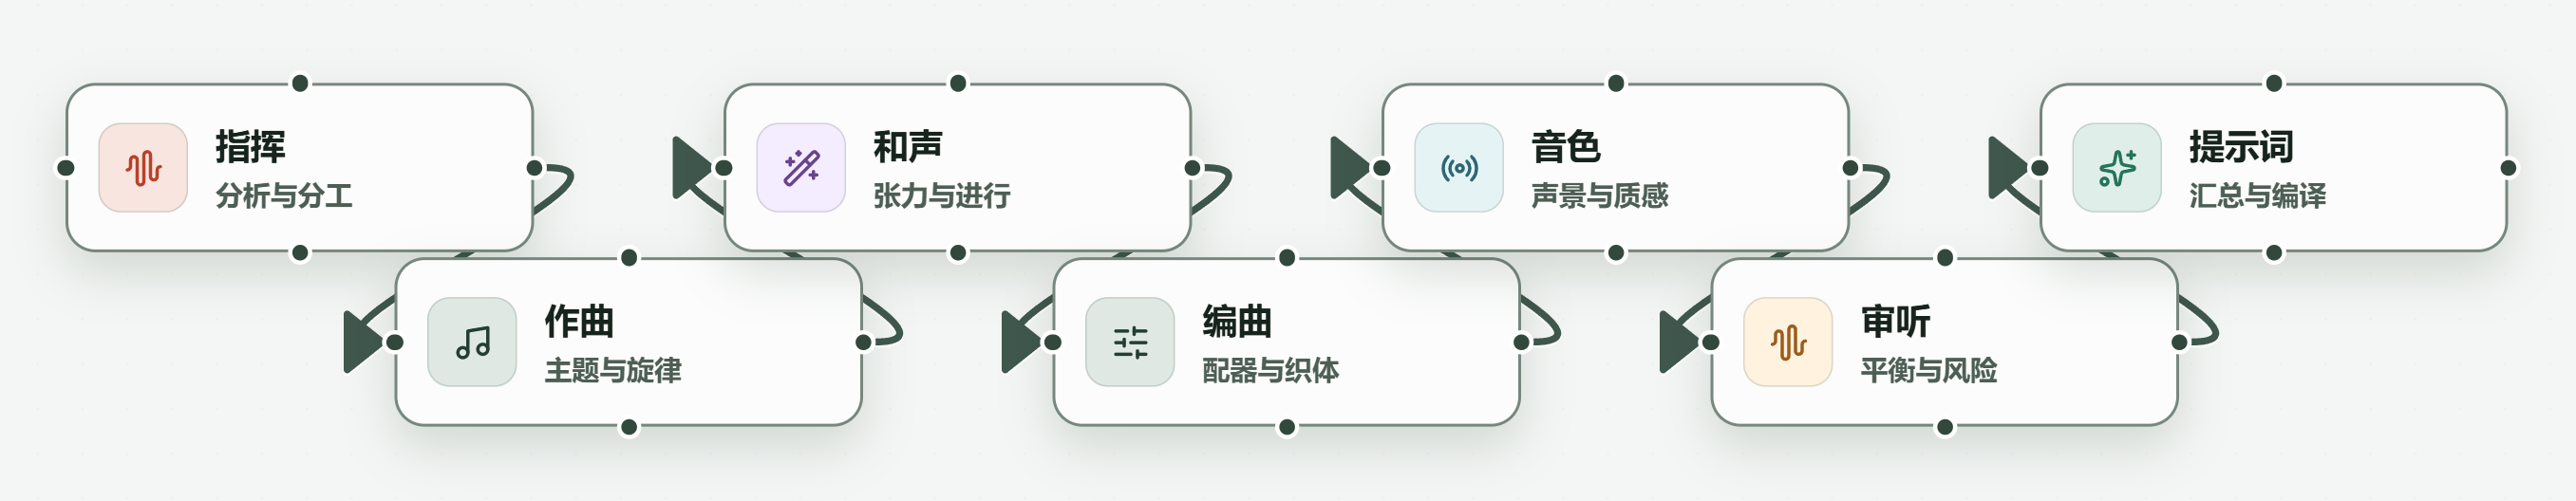
\includegraphics[width=\textwidth]{images/影视配乐编排.png}
    \caption{影视配乐工作流：围绕情绪叙事与空间声景组织节点}
    \label{fig:soundtrack-flow}
\end{figure}

\subsection{推理与规划方法}

\subsubsection{受约束的计划--执行}

Conductor Agent 相当于系统的任务规划器。它首先把自然语言需求整理成 CreativeBrief，再从固定枚举中选择工作流，并向后续角色下发细分指令。LangGraph 不执行模型任意生成的代码或节点名，而是将 \texttt{workflow} 映射到已注册的条件边。因此模型负责语义判断，程序负责执行合法性，形成受约束的 Plan-and-Execute。

以“创作一首雨夜氛围的电子纯音乐”为例，Conductor 应得到无人声、电子/氛围、夜色、慢至中速等简报，并选择 \texttt{electronic\_instrumental}；图执行先由 Rhythm 建立节奏骨架，再生成旋律与和声。若需求变为粤语摇滚，则必须选择含 Lyrics 的人声路径。这个规划过程解决了“同一任务模板无法兼顾所有音乐类型”的问题。

\subsubsection{工具调用式 ReAct}

上传参考音频后，Audio Reference Agent 使用 \texttt{bind\_tools} 接收三个白名单工具。模型观察资产名称和索引后决定调用探测、预览或波形工具；程序执行工具并把观察结果写回 \texttt{audio\_references}，供 Conductor 与 Arrange 使用。这一过程具有“观察--选择动作--取得工具结果”的 ReAct 特征，但工具参数只允许 \texttt{asset\_index}，模型无法提交任意本地路径。

与传统把文件内容直接塞进提示词相比，这种方式有两个优点：一是 ffprobe 返回的时长、采样率、声道等事实稳定可验证；二是模型的行动空间被限制在安全工具集内。系统同时在技能说明中规定，不得从元数据臆测准确和弦、歌词、艺人或配器。

\subsubsection{生成前反思}

Mix Review Agent 位于编曲与提示词编译之间。它不再创造新的主题，而是回看创意简报、旋律、和声、节奏、音色和编曲方案，重点检查人声与器乐冲突、低频拥挤、结构不清、风格漂移以及提示词过度堆砌。Prompt Compiler 再根据这份审听建议取舍内容。该步骤构成一次面向最终输出的 Reflection，使系统在调用付费或耗时的音乐服务前有机会发现全局问题。

\section{记忆机制设计}

\subsection{会话内短期记忆}

每个聊天 session 独立保存在 \texttt{data/sessions/<session-id>/session.json}，内容包括消息列表、摘要、上传资产和当前活动项目。南郭先生读取最近消息与 session 摘要，因此能够回答“这首歌是什么风格”“继续修改上一首”等依赖当前语境的问题。会话之间相互隔离，删除会话时对应资产一并移除。

图~\ref{fig:short-memory} 中，用户在作品完成后追问“这首歌的风格是什么”，系统能够从当前会话内已关联的运行结果回答港式摇滚、配器和情绪信息，说明短期上下文不只是保留聊天文字，也把作品运行与对话关联起来。

\begin{figure}[H]
    \centering
    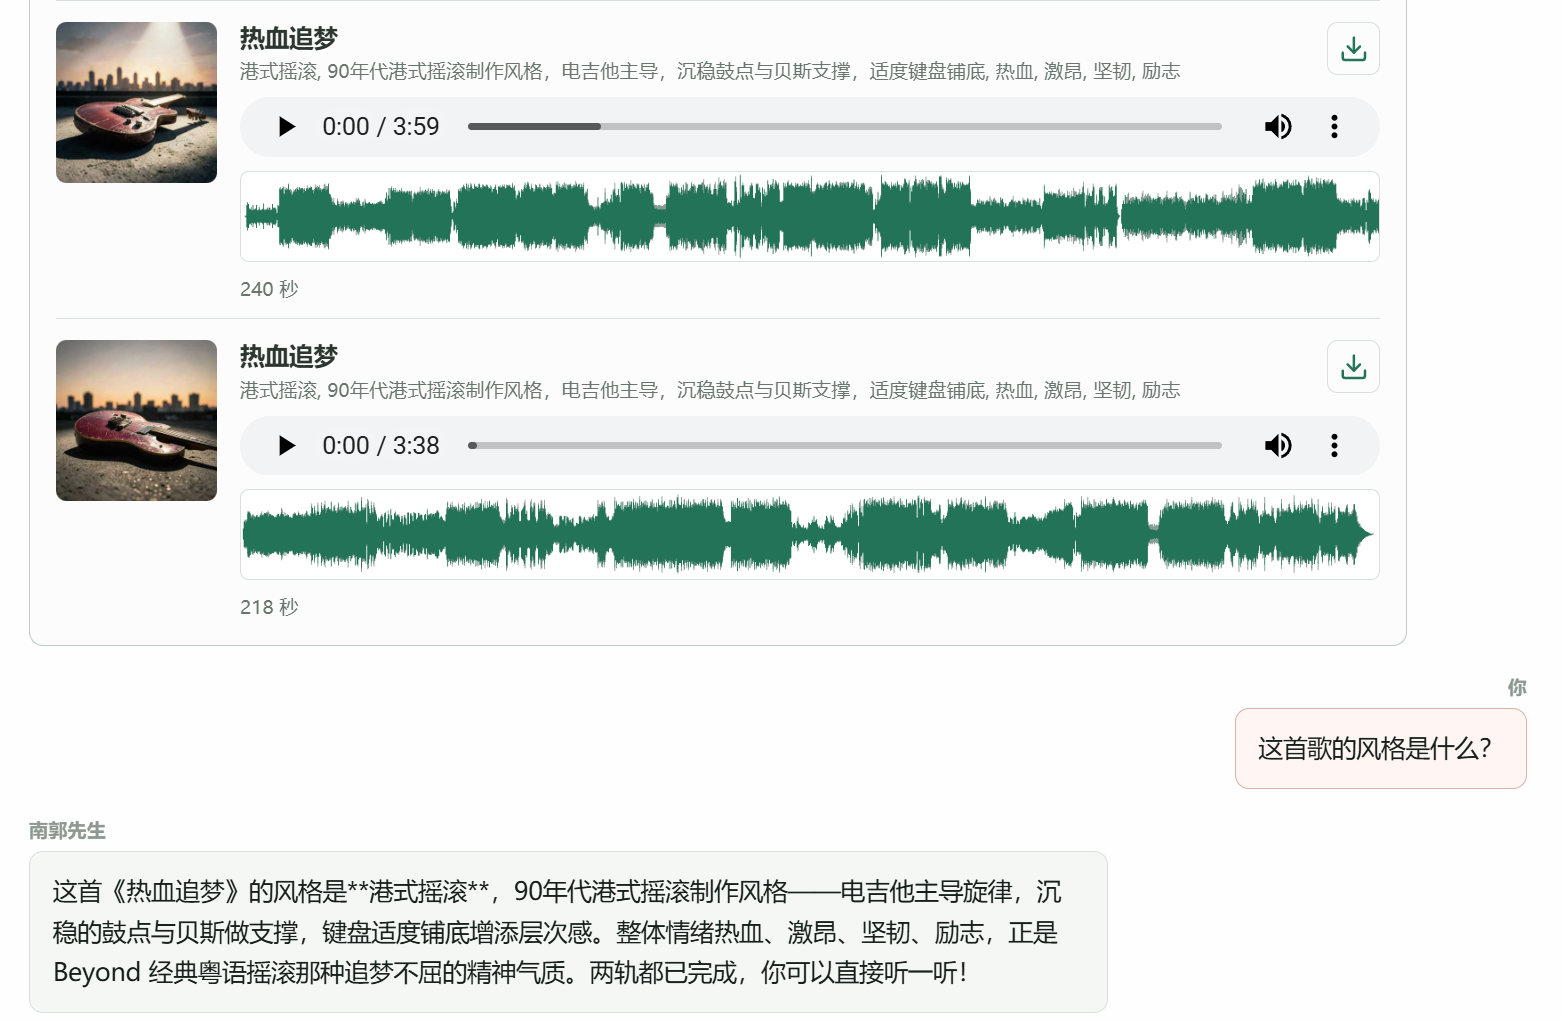
\includegraphics[width=0.88\textwidth]{images/会话内短期记忆.png}
    \caption{会话内短期记忆：根据当前作品回答后续问题}
    \label{fig:short-memory}
\end{figure}

\subsection{跨会话长期记忆}

长期画像存储在 \texttt{data/memory/user\_profile.json}，主要包含三类信息：

\begin{itemize}
    \item \textbf{语义记忆}：人声/器乐、偏好或避开的乐器、语言、流派、默认时长和制作风格等规范化偏好；
    \item \textbf{行为记忆}：各预设工作流完成次数，用于表现创作习惯；
    \item \textbf{情景记忆}：最近项目和作品的索引。音频事实仍以项目目录为准，画像只引用而不复制大文件。
\end{itemize}

Chat Agent 只提交用户明确表达的 MemoryObservation；MemoryStore 再做 key 规范化、value 归一化、去重与冲突替换。同一偏好被重复确认时增加证据次数并提高置信度；同一 key 出现新的明确值时替换旧值。写入采用临时文件原子替换，避免半写入 JSON。图~\ref{fig:preference-write} 展示“以后使用英语作为创作语言”被识别并提示已记录；图~\ref{fig:memory-view} 则展示长期偏好、置信度、确认次数、工作流计数和最近作品，并提供编辑、单条删除与清空能力。

\begin{figure}[H]
    \centering
    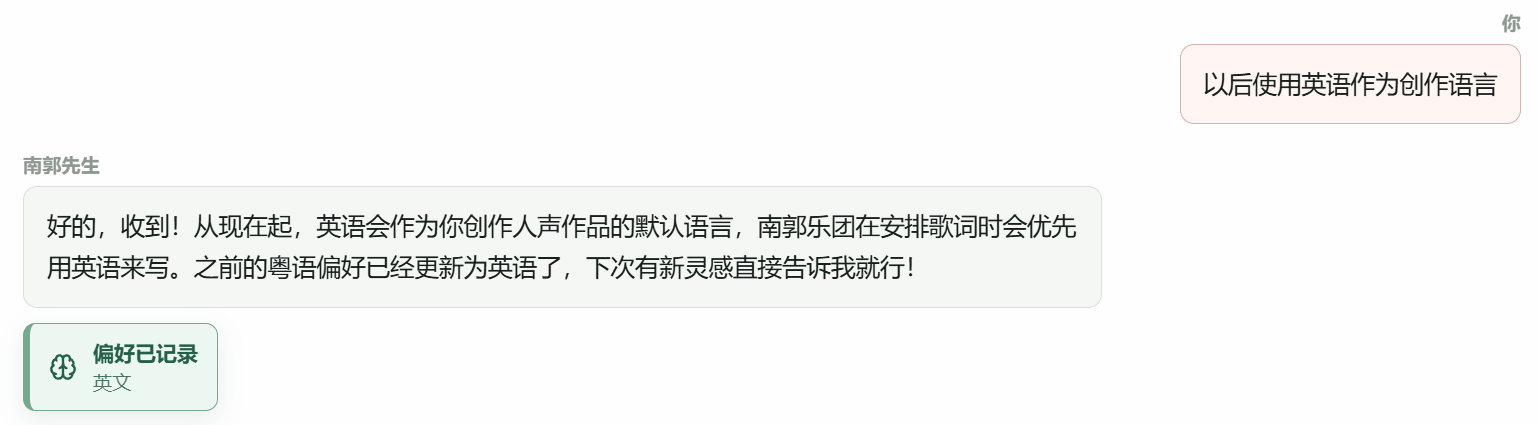
\includegraphics[width=0.9\textwidth]{images/记忆用户偏好（长期记忆）.png}
    \caption{从明确陈述中写入长期语言偏好}
    \label{fig:preference-write}
\end{figure}

\begin{figure}[H]
    \centering
    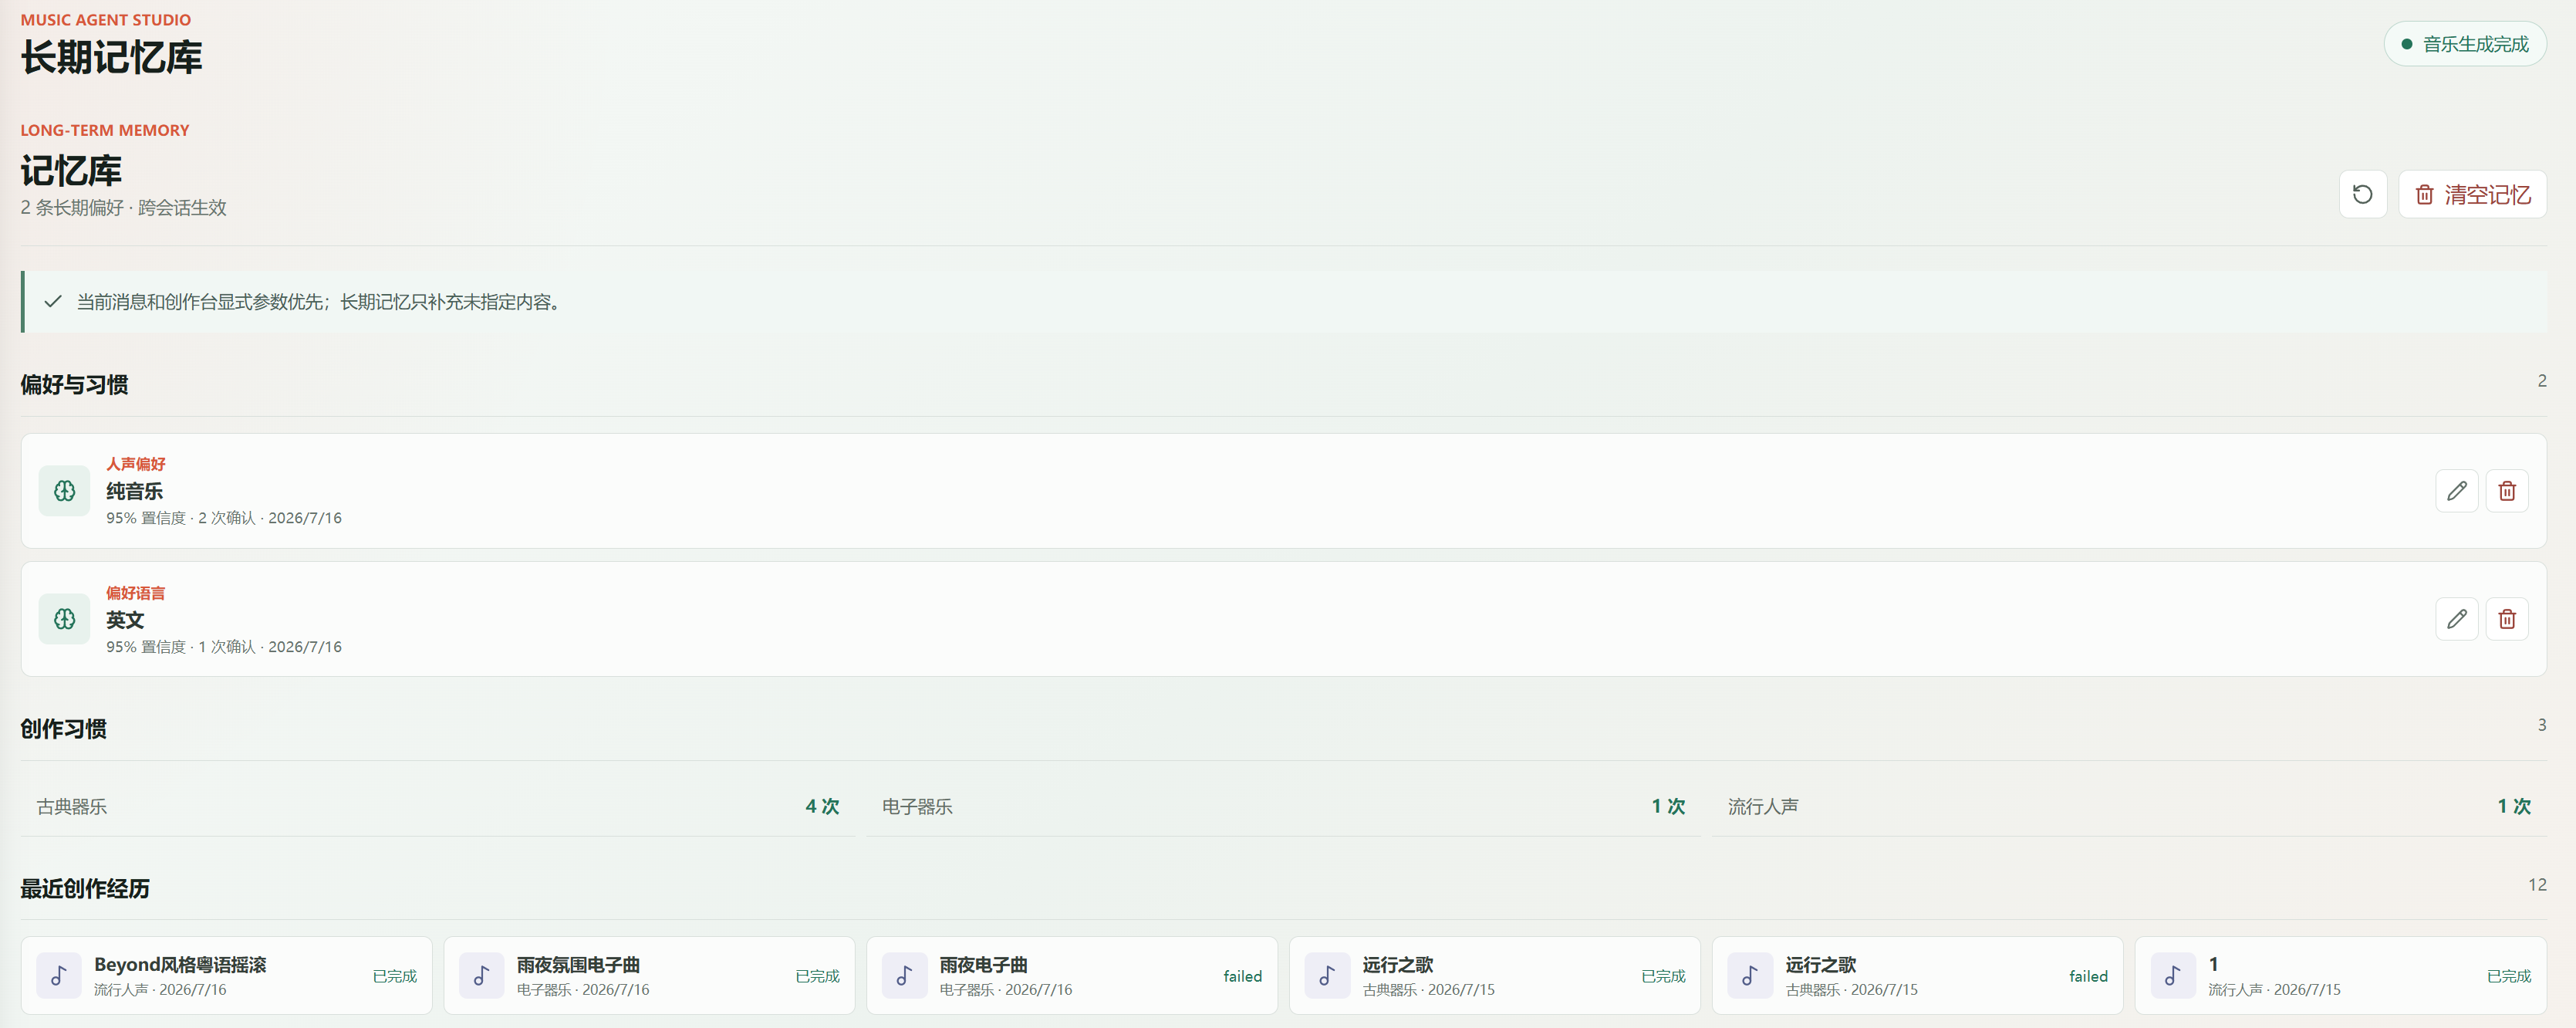
\includegraphics[width=\textwidth]{images/记忆库（长期记忆）.png}
    \caption{长期记忆库：偏好、创作习惯与最近经历}
    \label{fig:memory-view}
\end{figure}

\subsection{记忆冲突消解}

长期记忆只提供默认值，不能覆盖本次创作的明确要求。系统执行工作流前通过确定性函数解析 EffectiveCreativePreferences，其优先级为

\begin{equation}
P_{\mathrm{effective}} = P_{\mathrm{project\ control}}
\succ P_{\mathrm{current\ request}}
\succ P_{\mathrm{long\ term}}
\succ P_{\mathrm{default}} .
\end{equation}

其中项目预设可以直接确定人声属性；创作台明确选择的流派、语言和乐器优先；其次从当前文字中识别；只有未指定字段才读取置信度不低于 0.55 的长期偏好。系统还在 \texttt{sources} 中记录每个有效值的来源。图~\ref{fig:chat-conflict} 所示实验中，历史画像偏好“纯音乐”，但当前明确要求粤语歌曲，南郭先生选择人声路线，体现了当前意图优先。此规则避免了“记忆越多，系统越不听当前指令”的常见问题。

\begin{figure}[H]
    \centering
    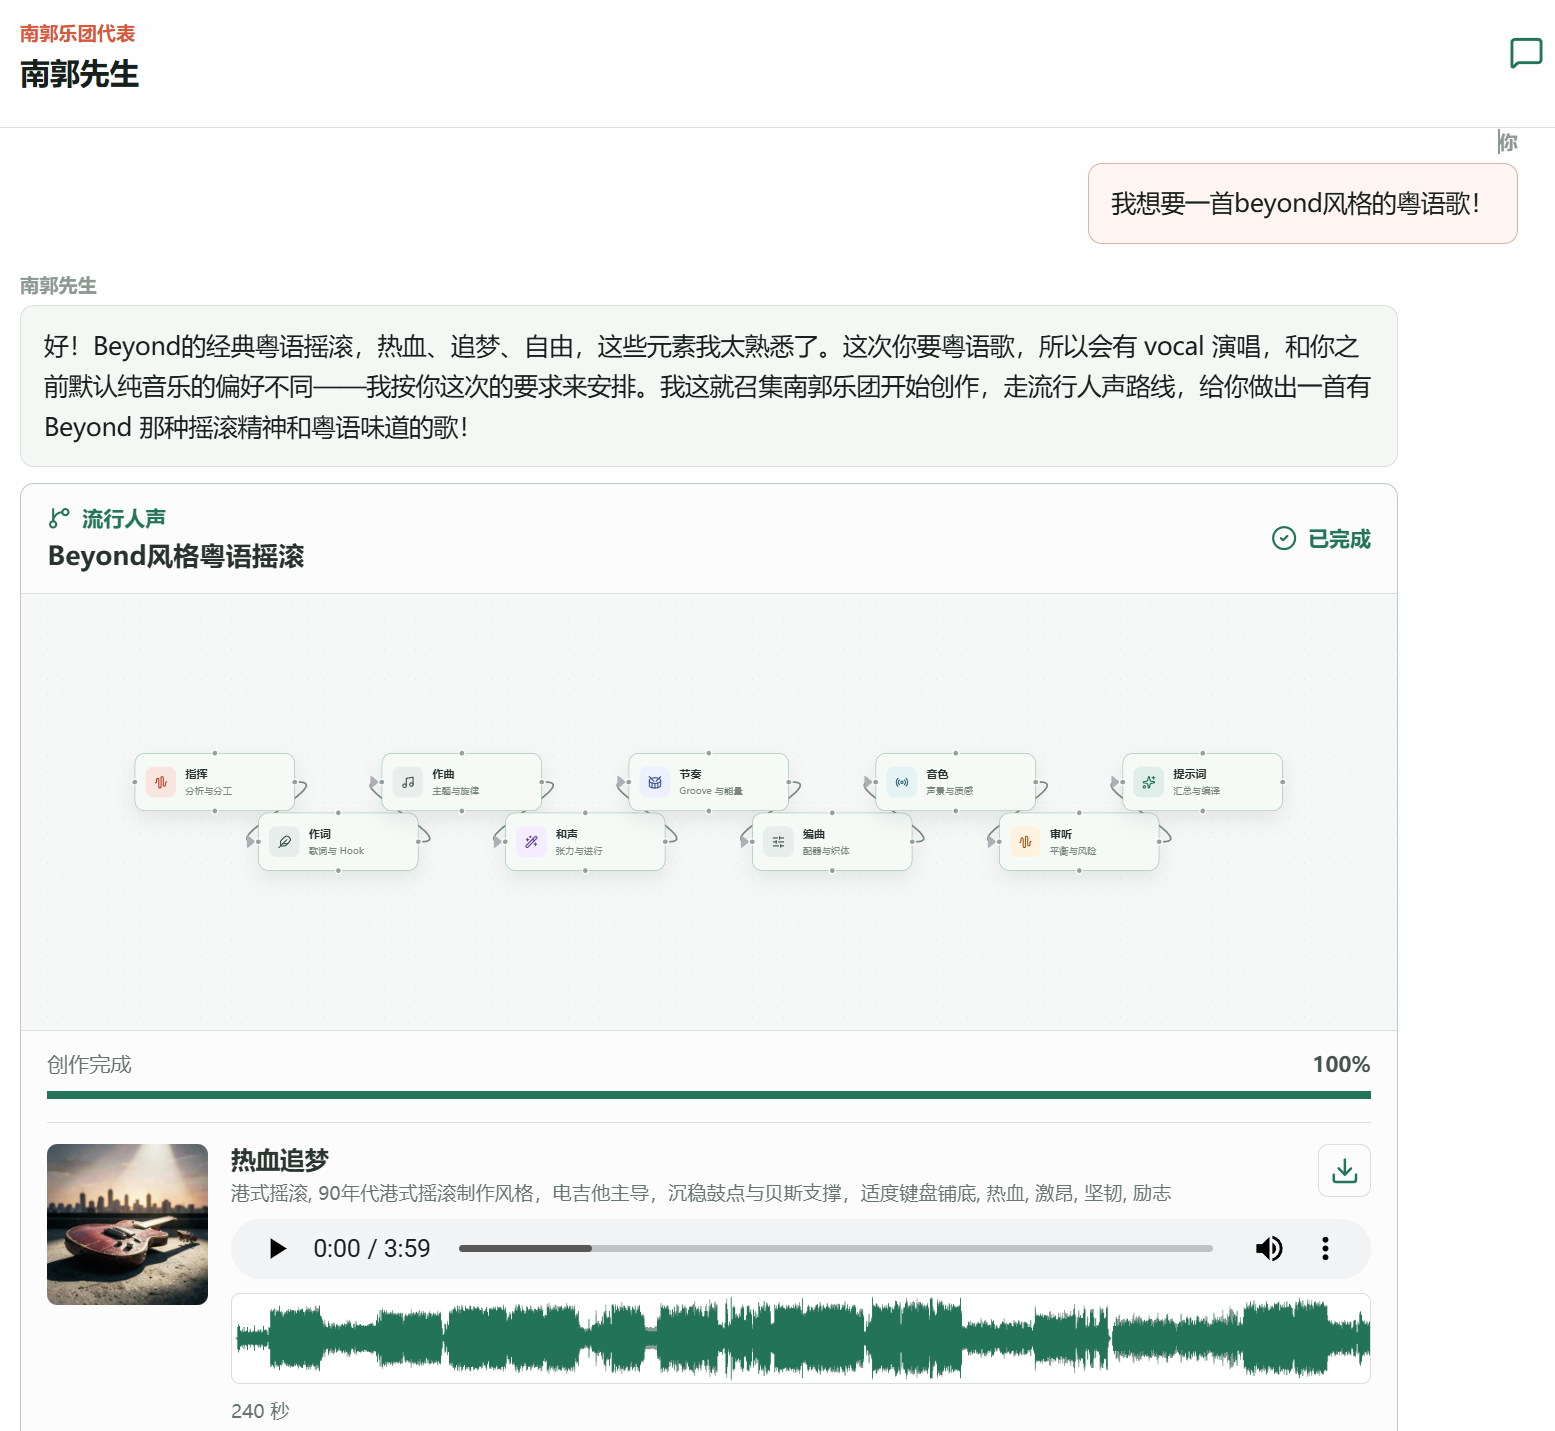
\includegraphics[width=0.82\textwidth]{images/与南郭先生对话.png}
    \caption{当前粤语人声请求覆盖历史纯音乐偏好}
    \label{fig:chat-conflict}
\end{figure}

\section{工具调用与外部能力}

\subsection{确定性工具分类}

系统将工具按输入输出性质划分为多类，既包含信息检索/探测，也包含计算、媒体变换和生成操作。

\begin{table}[H]
    \centering
    \caption{工具类型及其在工作流中的用途}
    \label{tab:tools}
    \begin{tabularx}{\textwidth}{L{3.0cm}L{4.2cm}Y}
        \toprule
        类型 & 工具 & 作用 \\
        \midrule
        音频探测 & \texttt{inspect\_audio} & 调用 ffprobe 返回时长、封装格式、编码、采样率、声道、码率和文件大小。 \\
        音频变换/可视化 & \texttt{trim\_audio\_preview}、\texttt{render\_waveform} & 生成响度规范化短预览和波形图片，支持参考分析与结果展示。 \\
        确定性音频合成 & \path{render_prompt_demo_audio} & 从提示词确定三个频率，合成 12 秒轻量和声音频，作为中间检查而非最终音乐。 \\
        乐谱计算与导出 & \texttt{build\_score}、\texttt{export\_score} & 由 ScoreSpec 构造 music21 Score，输出 MusicXML 与 MIDI。 \\
        外部音乐生成 & \path{KieSunoProvider.generate} & 提交结构化请求、轮询任务、下载音频和封面，并处理字段长度限制。 \\
        结果后处理 & \path{summarize_generated_audio} & 对下载音乐再次探测，并为每条作品产生波形与可展示的技术信息。 \\
        \bottomrule
    \end{tabularx}
\end{table}

图~\ref{fig:audio-input} 中，创作输入支持 MP3、WAV、FLAC、M4A 参考音频；文件进入项目资产目录后，Audio Reference Agent 只能凭索引调用工具。所有命令都以参数列表启动，不拼接 shell 字符串，同时设置超时并检查返回码，从而降低命令注入和挂起风险。

\begin{figure}[H]
    \centering
    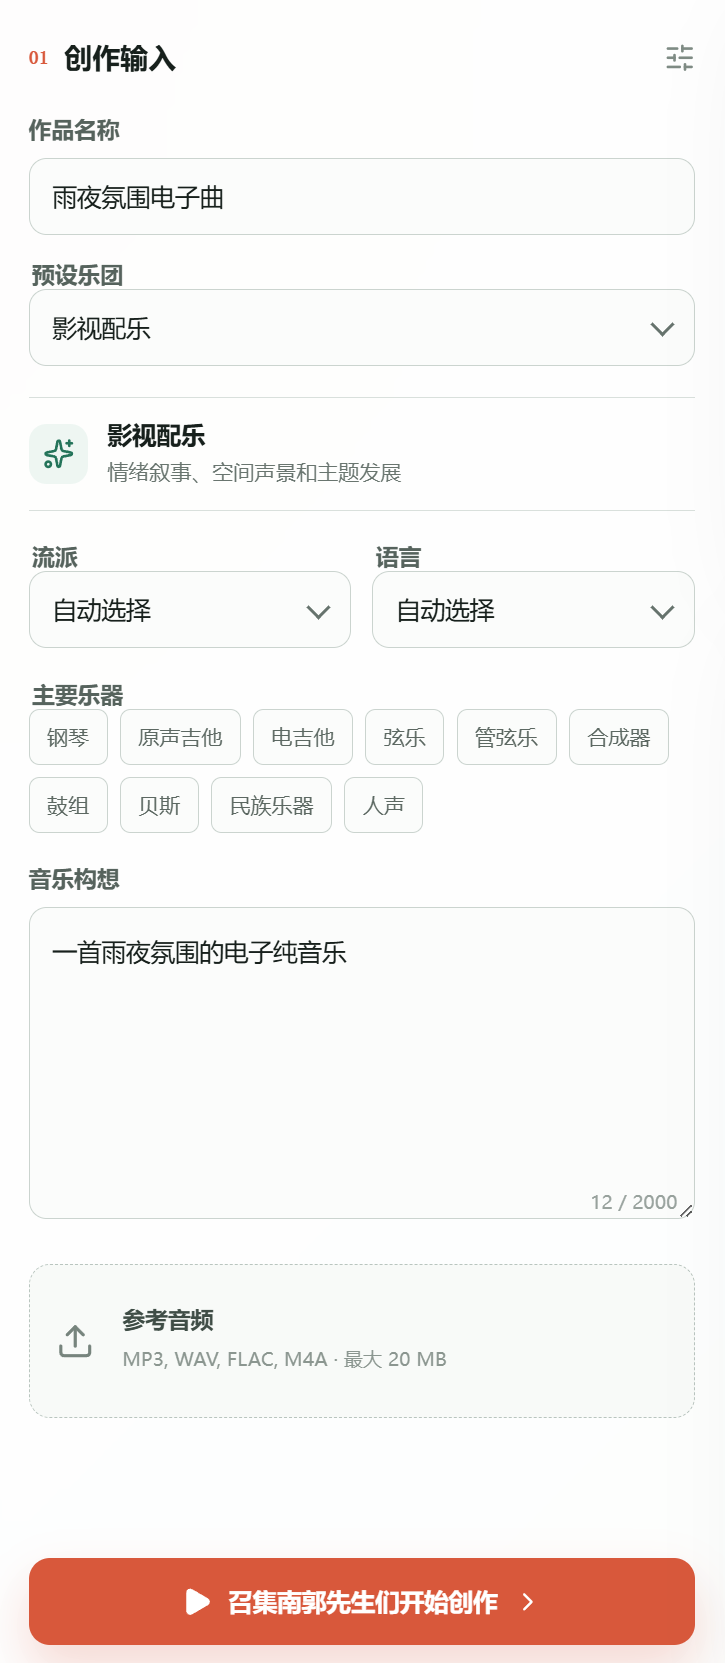
\includegraphics[height=0.72\textheight]{images/创作输入——可上传音频（工具调用）.png}
    \caption{创作输入与参考音频上传入口}
    \label{fig:audio-input}
\end{figure}

\subsection{乐谱与音乐生成边界}

古典器乐路径在 Melody Agent 提供 ScoreSpec 且项目存在 artifact 目录时，才进入 Score Export 条件节点。ScoreSpec 仅允许有限声部、合法速度、拍号、调号、音高、时值和力度，music21 再确定性地导出 \texttt{score.musicxml} 和 \texttt{score.mid}。因此大模型提出音乐结构，工具负责文件格式细节，缺少乐谱时不会阻断其他工作流。

Prompt Compiler 只负责编译音乐语义，不直接发送网络请求。KieSunoProvider 单独处理 API key、callback URL、模型字段长度、异步轮询、失败状态、文件安全命名、音频和封面下载。这种供应商隔离使未来替换服务时无需修改作词、作曲或编曲 Agent。密钥与服务地址只从环境变量读取，也不会出现在最终提示词中。

\subsection{生成结果的可视化}

工作流得到最终提示词后，应用层先生成一个 12 秒、96 BPM 的本地 Demo，再调用音乐服务。下载完成后，每条曲目通过 ffprobe 读取元数据，并用 ffmpeg 渲染波形。图~\ref{fig:audio-result} 显示同一任务返回两条约 4 分钟音频，它们具有不同的能量分布；用户可播放、比较和下载。工具失败会记录 \texttt{demo\_audio\_error} 或 \texttt{generated\_audio\_analysis\_error}，但后处理失败不会抹去已经成功下载的主音乐。

\begin{figure}[H]
    \centering
    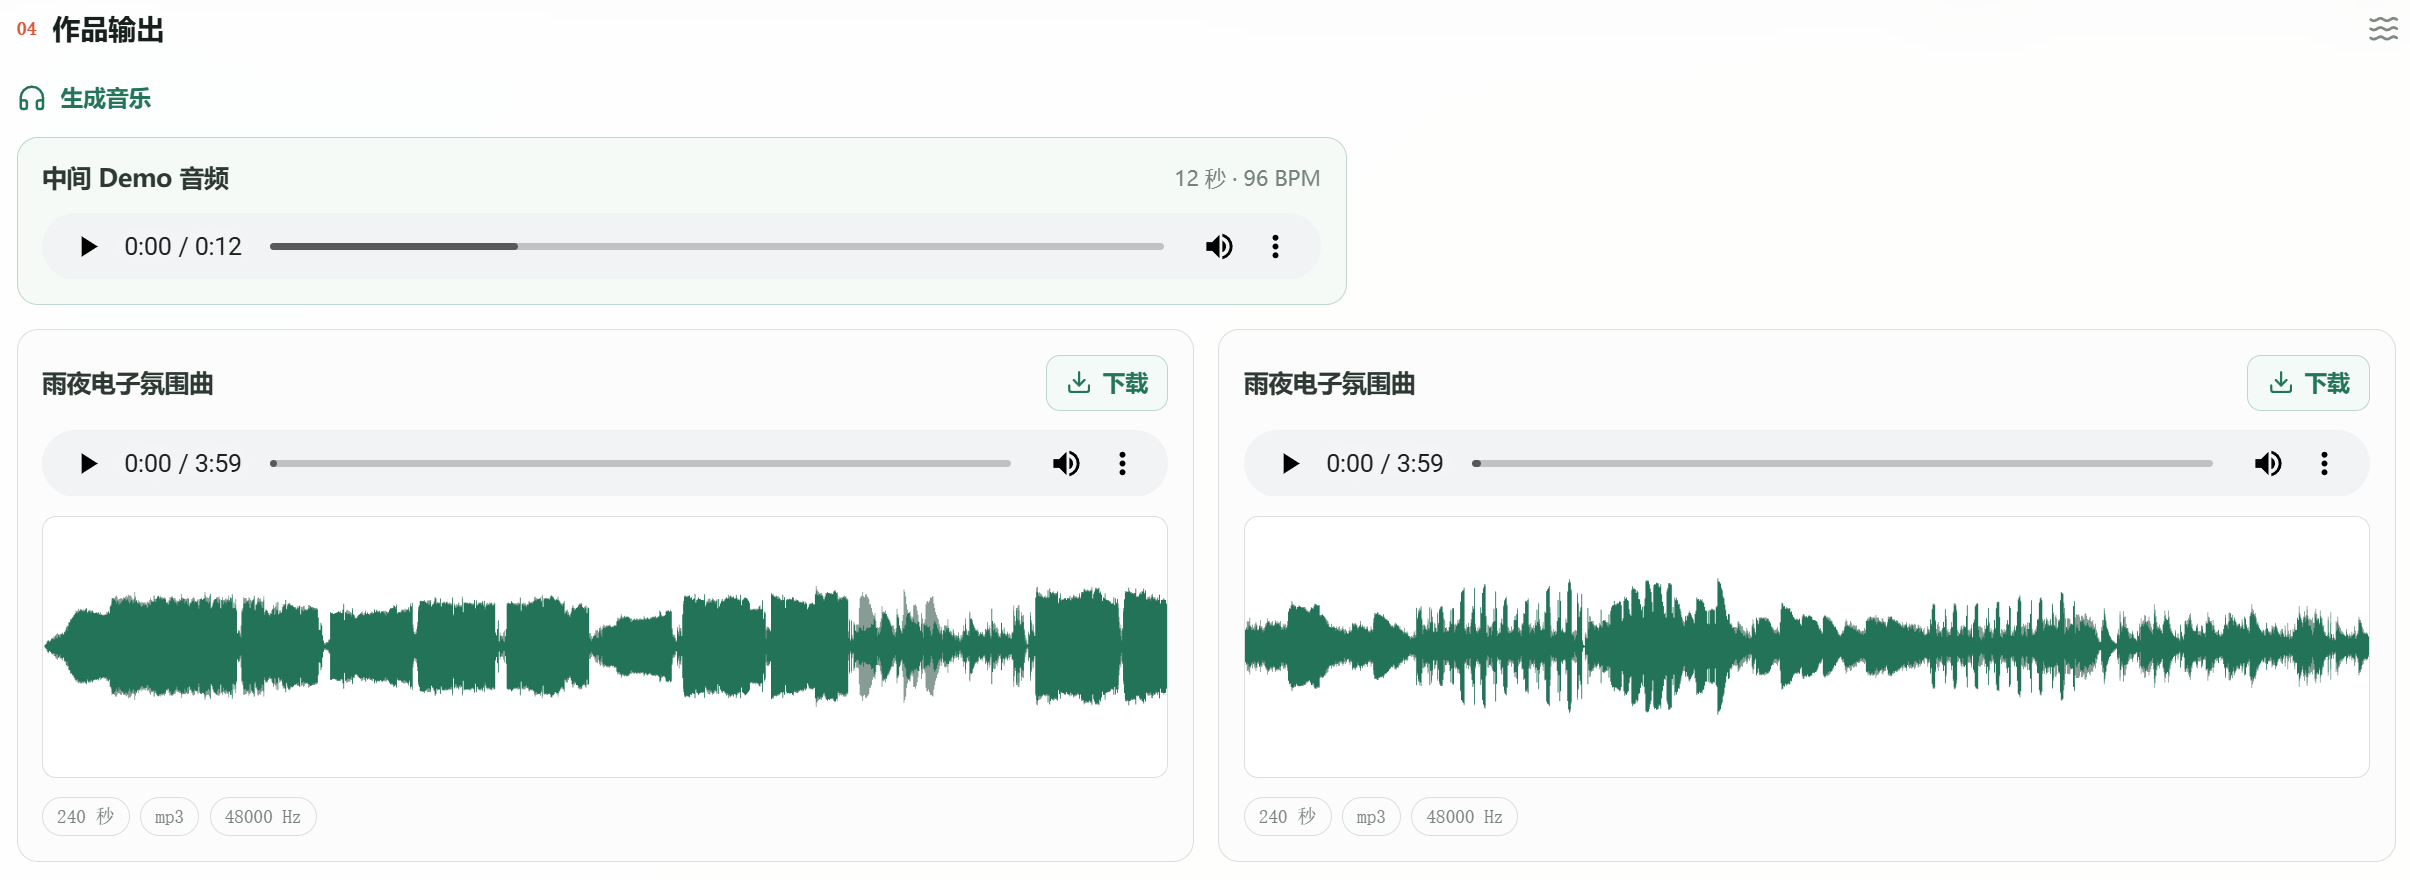
\includegraphics[width=\textwidth]{images/音乐生成可视化（工具调用）.png}
    \caption{中间 Demo、最终音乐和波形可视化}
    \label{fig:audio-result}
\end{figure}

\section{应用实现与本地数据管理}

\subsection{FastAPI 运行生命周期}

FastAPI 提供会话、记忆、项目、上传、同步/异步运行和作品集接口。长时间音乐生成采用本地后台线程：请求创建 Run 后立即返回 run id，前端轮询状态；后端依次把进度更新为 workflow、demo\_audio、music\_generation、audio\_analysis 和 completed。任一步骤抛出异常时，Run 持久化 failed 状态、阶段和可操作错误；服务重启还会把遗留的 running 状态恢复为中断失败，避免界面永久显示“生成中”。

\noindent\textbf{代码 2：工作流执行的关键阶段（节选）}
\begin{minted}{python}
effective = memories.resolve_preferences(project)
result = graph.invoke({
    "user_request": workflow_request(project, effective),
    "preset": project.preset,
    "effective_preferences": effective,
    "reference_audio_paths": reference_paths,
})

result["demo_audio"] = build_prompt_demo_audio(final_prompt, ...)
tracks = music_generator(final_prompt, ..., **generation_options)
result["generated_tracks"] = [generated_track_payload(t, ...) for t in tracks]
result["generated_audio_analysis"] = analyze_generated_tracks(tracks, ...)
\end{minted}

为保持本地实验实现简单，系统用一个 workflow lock 串行保护生成执行，不引入消息队列。这个选择适合单用户课程实验：状态更容易理解，也避免多个耗资源任务并发；代价是多个请求需要排队，后续若扩展多用户服务需改为任务队列或基于进程的执行器。

\subsection{文件系统持久化}

项目数据按目录组织，无需数据库：

\begin{minted}[linenos=false]{text}
data/projects/<project-id>/
  project.json
  assets/
  artifacts/score.musicxml, score.mid
  runs/<run-id>.json

data/sessions/<session-id>/session.json, assets/
data/memory/user_profile.json
works/<generated audio, cover, waveform, demo>
\end{minted}

LocalProjectStore、LocalSessionStore 和 LocalMemoryStore 分别成为各自目录结构的唯一管理入口，并在保存 JSON 时先写临时文件再原子替换。运行日志写入 \texttt{\_logs/}，涵盖 API 阶段、Agent 结构化输出、音乐任务提交/轮询和关键错误；数据、音频、密钥与日志均不提交仓库。

\subsection{前端交互闭环}

前端不是只展示最终一段文本，而是围绕用户任务提供四个相互衔接的页面：

\begin{itemize}
    \item \textbf{对话页}：自然语言讨论、上传参考音频、创建/修改作品并在消息内查看生成进度；
    \item \textbf{创作台}：使用精确表单控制预设、流派、语言、乐器和构想，显示工作流画布与阶段；
    \item \textbf{作品集}：聚合已完成及生成中的作品，提供封面、风格、时长、播放和下载；
    \item \textbf{记忆库}：管理偏好、习惯和最近经历，允许用户纠正或清空记忆。
\end{itemize}

图~\ref{fig:portfolio} 中作品集以最近作品为主视觉，下方排列全部曲目。它读取本地 Project 与最新 Run，而不是另建一份可能过期的数据副本，因此对话中的作品、创作台输出和作品集保持一致。

\begin{figure}[H]
    \centering
    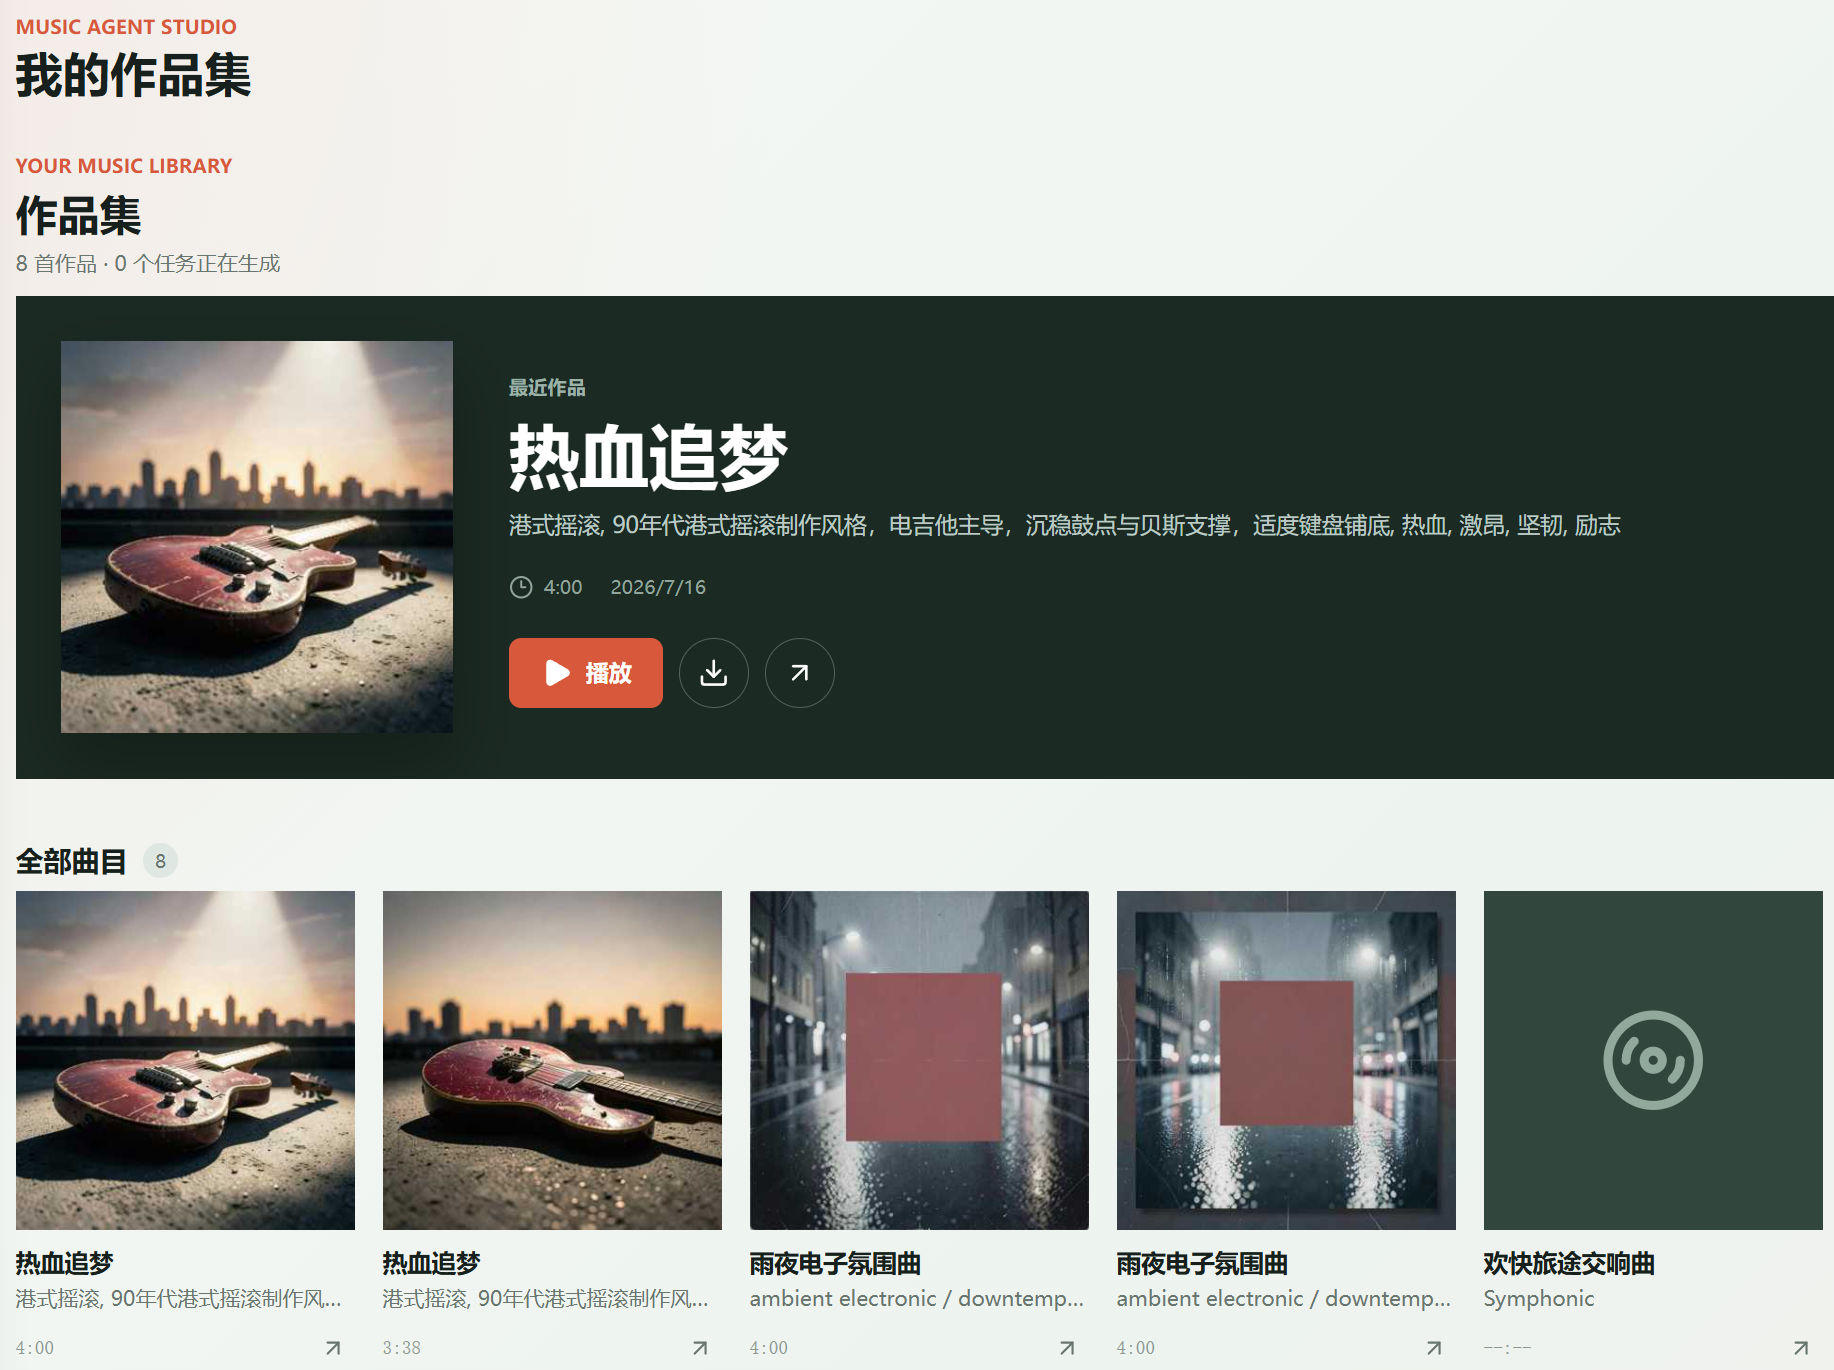
\includegraphics[width=\textwidth]{images/作品集.png}
    \caption{本地作品集与作品恢复入口}
    \label{fig:portfolio}
\end{figure}

\section{实验过程、结果与分析}

\subsection{实验环境与方法}

后端在 Python 3.12 环境下使用 uv 管理，前端使用 Node.js/npm；默认由根目录 \texttt{./start.sh} 同时启动 FastAPI（127.0.0.1:8000）和 Vite（127.0.0.1:5173）。LLM 使用 OpenAI Chat Completions 兼容接口，结构化输出方式可在 function calling、json schema、json mode 与 prompt JSON 间切换；真实音乐生成由配置 KIE API 的 Suno 兼容 provider 完成。

实验采用任务场景覆盖法，不只检查单个 Agent 的文本，而是观察路由、状态交接、工具产物、记忆冲突和作品持久化。主要用例如表~\ref{tab:cases}。

\begin{table}[H]
    \centering
    \caption{实验用例与观察点}
    \label{tab:cases}
    \begin{tabularx}{\textwidth}{L{1.2cm}L{4.0cm}Y}
        \toprule
        编号 & 输入场景 & 预期观察 \\
        \midrule
        E1 & 流行/摇滚人声作品 & 路径包含 Lyrics，生成内容包含语言和 Hook，最终可播放。 \\
        E2 & 电子纯音乐 & Rhythm 先于 Melody；不进入 Lyrics；生成中间 Demo、两条音频和波形。 \\
        E3 & 嘻哈人声与影视配乐 & 嘻哈路径由 Rhythm 先建立 beat，再进入 Lyrics 并包含 Performance；影视路径跳过 Lyrics。 \\
        E4 & 已记录纯音乐偏好后要求粤语人声 & 当前明确请求覆盖长期偏好，选择人声工作流。 \\
        E5 & 明确提出以后使用英语 & 写入/替换语言偏好，记忆库显示值、置信度和证据次数。 \\
        E6 & 上传参考音频 & 只能按资产索引调用探测/预览/波形工具，不允许任意路径。 \\
        E7 & 作品完成后追问与恢复 & 会话内可回答作品信息，作品集可继续播放和下载。 \\
        \bottomrule
    \end{tabularx}
\end{table}

\subsection{工作流差异实验}

E1 中，流行人声任务的画布由指挥进入作词，再逐步进入作曲、和声、节奏与编曲，说明歌词不是在最后附加的一段文本，而是旋律与编曲的上游状态。E2 中，雨夜电子纯音乐自动选择电子器乐乐团，节奏节点提前建立 Groove，完整工作台显示状态经历建档、参考、生成和完成；最终获得一个 12 秒 Demo 与两条 3:59 音频。E3 进一步体现了路径顺序的领域差异：嘻哈人声在作词前先建立 beat 和能量曲线，并通过 Performance 约束 flow、动态与人性化；影视配乐则正确跳过 Lyrics，避免器乐提示词混入演唱要求。

这些结果说明条件图能够根据任务改变分工顺序，而不是所有 Agent 无条件运行。角色复用也控制了实现复杂度：例如同一个 Harmony Agent 可在流行、古典、电子和爵士中工作，但其读取到的上游状态与指挥指令不同。另一方面，当前前端对古典与影视的核心节点展示较相似，尚未把 Score Export 等后端可选节点直接显示出来，用户对两者细粒度差异的感知仍可增强。

\subsection{记忆实验}

E4 的对话结果明确指出“这次要粤语歌，所以会有人声演唱”，并选择流行人声路径，没有机械继承历史的纯音乐偏好。E5 中，用户将默认语言从粤语修改为英语后，界面给出“偏好已记录”，长期记忆库显示英语及置信度；该修改会影响以后未指定语言的人声作品，但不会覆盖下一次显式选择的中文或粤语。

E7 中，用户对刚完成作品进行追问，系统能够结合 session 内的 workflow run 返回风格、配器与情绪；跨会话后，作品仍可在作品集中发现。由此可见短期记忆负责连续对话，长期记忆负责稳定偏好，项目文件负责作品事实，三者没有混为一个无限增长的聊天历史。

\subsection{工具与产物实验}

E6 验证了参考音频上传入口和受限工具调用。工具结果是结构化技术事实，并可生成可供人工检查的预览和波形。最终生成阶段又使用另一组确定性能力：本地 Demo 合成、外部音乐生成、下载音频探测和波形渲染。图~\ref{fig:audio-result} 中两条曲目波形形态明显不同，说明界面不仅返回两个链接，也提供了快速比较段落能量的视觉依据。

需要注意，当前 Demo 是根据提示词字符确定频率后混合三个正弦音的轻量参考，只能证明工具链、格式和播放界面正常，不能代表 Melody Agent 旋律计划的真实试听；参考音频工具也主要提供元数据和宏观波形，尚不具备调性、和弦、节拍或乐器识别能力。因此实验结果应解释为“多智能体与工具链完整可执行”，而不是“系统已经达到专业音频理解与编曲质量”。

\subsection{自动化验证}

项目针对图路由、结构化 Agent、API、记忆、provider、乐谱、技能加载、日志和音频工具提供了聚焦测试；外部 LLM、音乐服务和音频命令在测试中使用 fake 或 mock，不产生真实付费请求。前端还提供 lint、production build 和 Playwright 工作区测试。验证命令如下：

\begin{minted}[linenos=false]{bash}
uv run pytest
uv run python -m compileall -q agents app lib models main.py
npm --prefix frontend run lint
npm --prefix frontend run build
\end{minted}

实际验证中，后端共收集 55 个测试，覆盖 API、参考音频 Agent、图路由、结构化 LLM、日志、记忆、provider、乐谱、技能加载与音频工具，结果为 \texttt{55 passed}；前端 lint 与 production build 均成功，Vite 完成 1935 个模块转换。测试重点保证系统结构和失败处理的确定性；最终音乐的审美质量仍需要试听评价，不能由单元测试替代。

\subsection{综合结果评价}

\begin{table}[H]
    \centering
    \caption{实验结果的综合评价}
    \label{tab:evaluation}
    \begin{tabularx}{\textwidth}{L{3.0cm}L{3.0cm}Y}
        \toprule
        评价维度 & 实验结果 & 分析 \\
        \midrule
        角色定位 & 完成 & 对话、规划、音乐专业与供应商职责分离，输入输出受模型约束。 \\
        分工与流程 & 完成 & 八种预设复用节点并改变顺序，人声/器乐和爵士/嘻哈等路径有实质差异。 \\
        推理规划 & 完成 & 计划--执行负责全局路由，ReAct 负责工具选择，Mix Review 负责生成前反思。 \\
        长短期记忆 & 完成 & session 上下文与跨 session 画像分离，显式优先级规则避免历史覆盖当前。 \\
        工具能力 & 完成 & 覆盖音频探测、音频变换、波形、Demo、乐谱和外部生成，产物可视化。 \\
        端到端体验 & 完成 & 可从对话或创作台发起任务，查看进度，并在作品集中恢复结果。 \\
        音乐可控性 & 部分完成 & 结构与提示词可控，但最终声学细节仍依赖外部生成模型。 \\
        扩展与并发 & 有限制 & 白名单预设安全清晰，但尚未执行自定义工作流，生成任务当前串行。 \\
        \bottomrule
    \end{tabularx}
\end{table}

\section{问题反思与改进方向}

\subsection{参考音频理解仍偏浅}

现有 Audio Reference Agent 能可靠获得技术参数、预览和宏观能量图，却不能把音频转换为 BPM、调性、段落边界、和弦或配器标签。后续可增加 librosa/Essentia 等确定性分析工具，并让输出继续遵守 Pydantic schema；若增加语音转写或旋律转录，也应区分“检测事实”和“模型推断”，给出置信度而非把猜测写进创作状态。

\subsection{反思尚未形成闭环修订}

Mix Review 当前把风险建议传给 Prompt Compiler，但不会把问题退回 Harmony、Rhythm 或 Arrange 自动重写。它实现了一次轻量 Reflection，却不是多轮自我修正。后续可以把风险分级：一般问题由 Prompt Compiler 消化；关键冲突通过条件边返回对应节点，并限制最大重试次数，避免图循环失控和调用成本无限增长。

\subsection{风格模仿与内容边界}

实验截图中的用户直接指定了知名乐队风格，系统能够理解其摇滚、粤语、热血等意图，但界面回复仍复述了艺人名称。虽然 Prompt Compiler 已被要求不要模仿受版权保护的艺术家，入口层还应更早把专名转换为“年代、地域、配器、速度、情绪、制作质感”等可解释特征，并提示用户系统创作的是原创作品。这既提高提示词的可控性，也减少过度近似具体艺人的风险。

\subsection{本地架构的容量边界}

JSON 文件、后台线程和全局 workflow lock 使系统易于部署和调试，适合个人实验；但它们不适合多用户高并发。多个实例同时写同一目录也缺乏跨进程锁。若后续扩展，可在不改变 Agent 领域模型的前提下替换项目存储和任务执行层，同时保留 provider 与工具边界。本实验不提前引入数据库和队列，是对当前规模的有意识取舍。

\subsection{工作流与评价仍可扩展}

系统已预留受约束自定义工作流方向，但当前只能执行八种注册预设。后续应定义 JSON Schema，只允许引用系统节点类型，并在执行前检查入口、终点、必需字段与无环/有界循环条件。音乐质量评价还可加入人工盲听表，从主题一致性、结构完整性、音色契合度、歌词可唱性和重复生成稳定性等维度统计，而不只依赖界面成功状态。

\section{结论}

本实验完成了一个可本地运行的多智能体音乐创作系统。系统的关键价值不在于堆叠 Agent 数量，而在于把开放音乐任务转化为有边界的协作：南郭先生负责用户关系与记忆，Conductor 负责受约束规划，各音乐角色只更新自己的领域状态，Mix Review 在生成前做全局审查，Prompt Compiler 与 provider 分别承担语义编译和服务调用。LangGraph 条件边使八类音乐工作流能够复用角色并保持差异；短期会话、长期偏好与项目事实共同支持连续创作；多类音频、乐谱和生成工具则把语言规划落实为可播放、可视化、可下载的作品。

从实验结果看，系统已经形成“理解需求--规划分工--专业协作--工具执行--记忆沉淀--作品恢复”的闭环，并能在当前请求与历史偏好冲突时做出合理选择。其不足主要集中在参考音频的乐理理解、反思回路深度、并发扩展和风格安全抽象。上述问题均可在现有结构化状态和分层边界上渐进改进，而无需推翻当前架构。

\section{参考资料}

\begin{enumerate}
    \item LangChain AI, \textit{LangGraph Documentation}. \url{https://docs.langchain.com/oss/python/langgraph/overview}
    \item Pydantic, \textit{Pydantic Documentation}. \url{https://docs.pydantic.dev/}
    \item FastAPI, \textit{FastAPI Documentation}. \url{https://fastapi.tiangolo.com/}
    \item React Flow, \textit{React Flow Documentation}. \url{https://reactflow.dev/}
    \item music21, \textit{music21 Documentation}. \url{https://www.music21.org/music21docs/}
    \item FFmpeg Project, \textit{FFmpeg Documentation}. \url{https://ffmpeg.org/documentation.html}
    \item theNanGuos 项目源码、架构说明、提示词与测试代码。
\end{enumerate}

\clearpage
\end{document}
